\documentclass{article}
\usepackage{amsmath}
\usepackage{mathtools}
\usepackage{txfonts}
\usepackage[margin=0.5in]{geometry}
\usepackage{graphicx}
\graphicspath{ {images/} }


\setlength{\parskip}{\baselineskip}%
\setlength{\parindent}{0pt}%

\title{STAT 672 Final Project}
\author{Daniel Hartig}


\begin{document}
\maketitle

\section{Introduction}

The purpose of this experiment is to create a method for estimating the ridership at a subway station based on demographic characteristics of the surrounding area. 

I chose two cities' subway system for use due to the similarity of the cities: Boston and Chicago. Both cities have similar population density in their downtown areas as well as similiar sized subway systems: Boston had 112 stations and 241 million yearly riders,Chicago had 136 stations and 238 million yearly riders. In addition, these cities have similar external features which might be expected to affect subway ridership: both cities subway systems are at least 100 years old and thus well established, and both cities have cold winters that might affect people's willingness to walk. 

Using the data available from online sources for these two cities, I calculated various 'features' of each subway station on the network, and then applied regression based machine learning to determine relationships between the features and measured subway ridership. Since ridership numbers vary depending on the day of the week, I used average weekday subway ridership as my target values. To support this choice, I used schedule values average between the morning and evening rush hours for each system to determine such characteristics as travel time between stations, and frequency of trains at each station. 

\section{Data Sources}

\subsection{Zip Code Data}

The data for this project comes from the US Census bureau and is available at factfinder.census.gov. Subway ridership during weekdays is driven primarily by commutes to work. A quick look at ridership data for the two cities shows the highest usage stations are located in the central business districts of their cities. To reflect the commute, I chose four basic data points: total population, number of households, total number of employees, and net pay of all employees. This includes two different statistics to measure where people live, and two others to measure where people work. 

In addition to the counts of the above data points for each zip code, each zip code has a land area. Dividing the counts by the land area gives us a density for each of the data points. Finally, each zip code has a geographical centroid associated with it, which is stored in the database. 

\subsection{Subway Station Data}

For each subway station, I obtained geographical coordinates for that station and ridership data. The ridership data came from self-reported numbers released in annual reports from the subway's operating agency (Massachussets Bay Transportation Authority for Boston; Chicago Transit Authority for Chicago). I searched for the geographical coordinate myself and recorded them using Google Maps. 

Also included is a parking flag. This boolean is true if there is parking available at the station, as indicated by the respective transit authority, and false if there is no parking available.

\subsection{Estimates of Density}

For each station, I estimated the average density within 1 km of the station for each of the data points. I accomplished this in a two step process: first I found out the zip codes close enough to the station to be important for calculating its density, then made a weighted average density where the weights were the inverse of the distance from the station to each zip code.

Zip codes have irregular shapes, and geographical data for them is given by centroid, so it is hard to determine exactly what portion of which zip codes are within a certain radius of a station. To determine estimate if a zip code was close enough, I used a two part filter. First I wanted to see if the zip code was close enough and large enough to be within 1 km of the station. I determined this by using the square root of that zip code's area plus the radius of the station's area (1 km) as a 'proximity statistic,' and determined if this was less than 1/2 of the distance between station and zip code's centroid. Second, I wanted to see if there were any other zip codes between the station and the zip code. To check this, I projected the vector connecting the station to this zip code onto all other closer zip code's vectors. I used the maximum projection subtracted from the the square root of the zip code's area as a 'blocking statistic' and determined if this was less than 1/3 of the distance between station and zip code. The factors 1/2 and 1/3 were determined experimentally by checking the results of this 'nearest zip code' algorithm against a map.

The results of this nearest zip code approximation are shown in tabular form for Sullivan Square station in the Charlestown neighborhood in Boston.

\begin{center}
\begin{tabular}{ c c c c c c c }
Zip Code & Distance to Station & sqrt(area) + 1& Large and Close & Projection & sqrt(area) + 1 - Proj & Not Blocked \\
\bf{02145} & 1.35 & 2.90 & True & N/A & 1.9 & True \\
\bf{02129} & 1.36 & 2.87 & True & -1.30 & 3.17 & True \\
\bf{02141} & 1.59 & 2.29 & True & 0.11 & 1.18 & True \\
\bf{02143} & 1.64 & 3.00 & True & 1.05 & 0.95 & True \\
02114 & 2.41 & 2.08 & True & 2.02 & -0.94 & False \\
02142 & 2.54 & 1.84 & True & 2.51 & -1.67 & False \\
\bf{02149} & 3.05 & 2.98 & True & 0.85 & 2.13 & True \\
02108 & 3.08 & 1.46 & False & N/A & N/A & N/A \\ 
02139 & 3.18 & 3.00 & True & 2.86 & 0.14 & False \\
\end{tabular}
\end{center}

\begin{center}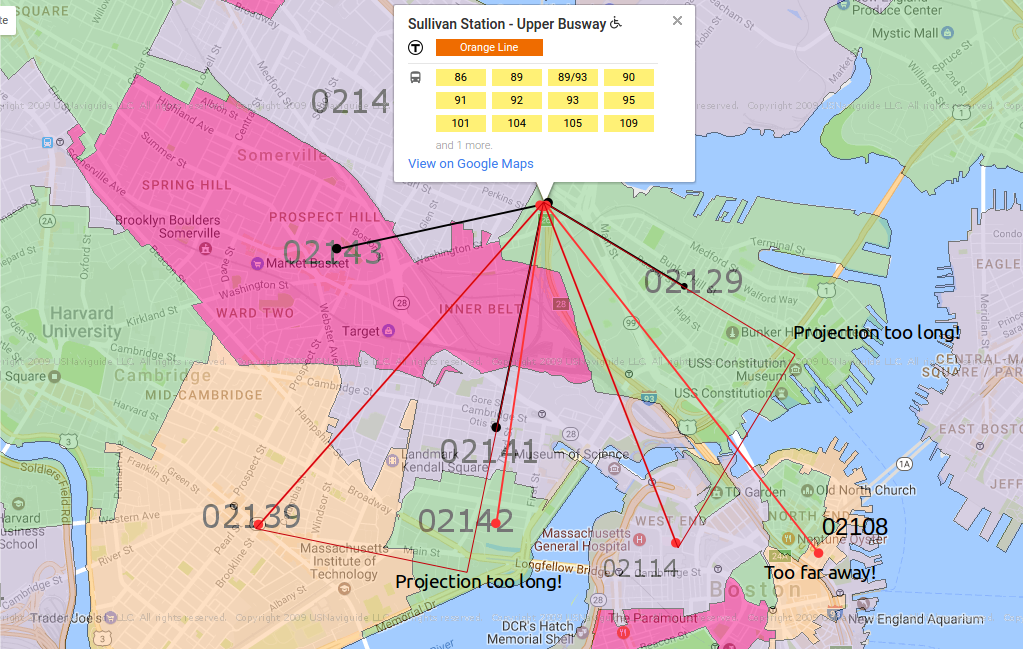
\includegraphics[scale=0.6]{Sullivan_for_distance_with_markup}\end{center}

We can see that five zip codes are accepted (02145, 02129, 02141, 02143, 02149; in bold). Several others (02114, 02142, 02139) are close enough and large enough to be considered, but they are 'blocked' by a closer zip code. For 02108 and other farther zip codes, they do not meet the close enough and large enough criteria, and so their projections are not even calculated. 

The next step to density calculation is to calculate the data density for the five selected nearby zipcodes and take the weighted average of them. 

\begin{center}
\begin{tabular}{ c c c c c }
Zipcode & Distance & Inverse Distance & Density & Weighted Density \\
02145 & 1.35 & 0.74 & 7036 & 5211 \\
02129 & 1.36 & 0.74 & 4707 & 3461 \\
02141 & 1.59 & 0.63 & 7186 & 4519 \\
02143 & 1.64 & 0.61 & 6156 & 3753 \\
02149 & 3.05 & 0.33 & 4682 & 1535 \\
\end{tabular}
\end{center}

\begin{center}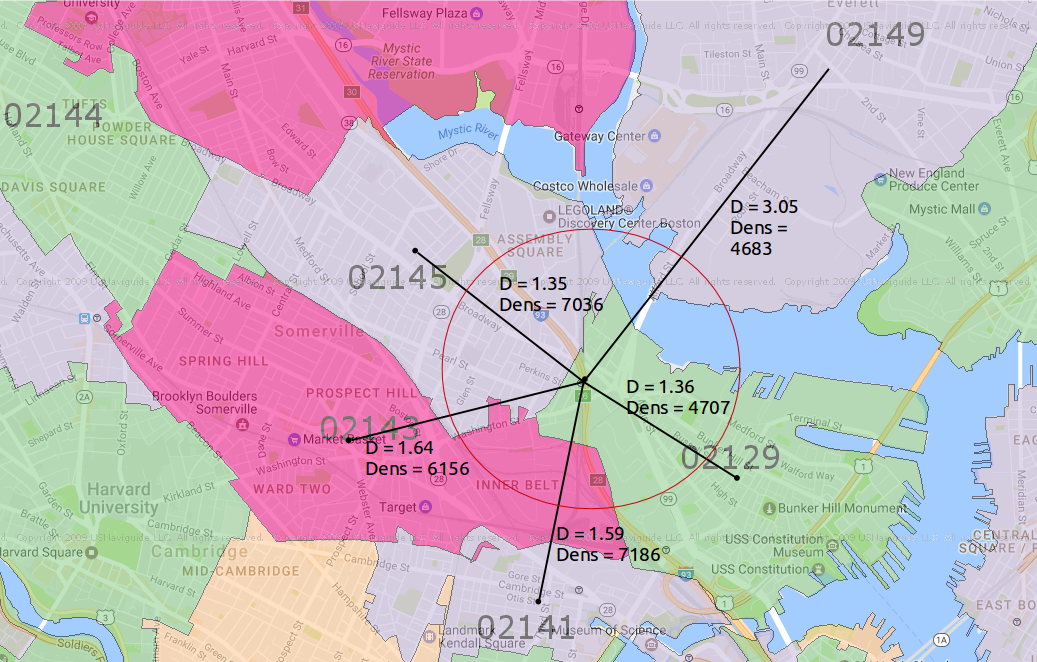
\includegraphics[scale=0.6]{Sullivan_for_density_with_markup}\end{center}

Dividing the summed weighted densities by the summed inverse distances gives a density estimate of 6074. While the estimate appears to be a good fit, the red circle at 1 km shows the drawbacks of this method. While 02141's centroid is closer to Sullivan Station than 02143 is; because od the orientation of the two zip codes, the station's 1 km radius circle overlaps with 02143 but not 02141. 

\subsection{Estimates of Area}

I chose four different geographic interpretations for each of the four data points for each data point: the count within walking distance; the count within walking distance where this station was the nearest; the count within driving distance; and the count within walking distance of a certain minute ride from the station. 

To calculate walking distance, I assume that 1 km was the farthest that from a station that a person was willing to walk. I then drew a 1 km circle around each station, and sampled 10,000 points chosen randomly from it. These points I compared against a shapefile of the state's geography to see if the points were on land or in water. The percentage of points found to be on land I multiplied by the area of the 1km circle ($\pi$ km$^2$) to obtain the area within walking distance of each station. This will be referred to as the 'walking' data for a station.

To calculate the area that was both within walking distance and also closest to this station, I used a similar method. I drew the same circle and sampled 10,000 points, but in additon to checking against a shapefile to determine if the point was on land, I used a geographic r-tree index of station to determine if any other station was closer to this point the the station of interest. The number of points that were both on land and closest to the station of interest is then divided by 10,000 and muliplied by the area of the walking distance circle to get total area nearest to that station. This will be referred to as the 'nearest' data for this station.

In this example, the green dots are counted as good, while the red dots are closer to some other station and the blue dots are in the water. Out of 100 dots, 75 are green, 15 are red, and 10 are blue. The calulated 'walking' area includes the green and red dots and is 90\% of the area of the 1 km radius circle; the calculated 'nearest' area includes only teh green dots and is 75\% of the 1 km radius circle. 

\begin{center}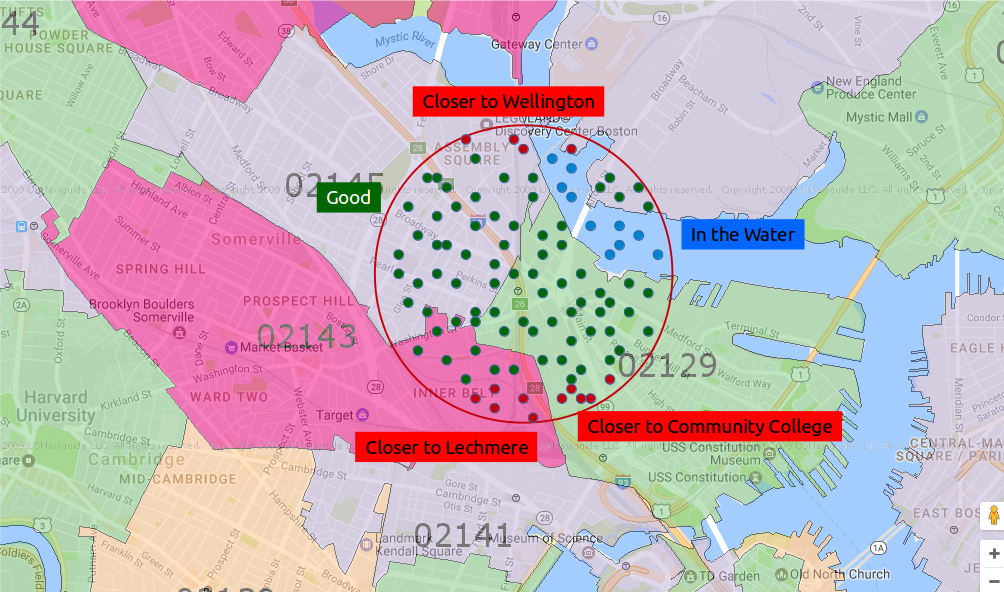
\includegraphics[scale=0.6]{area_with_markup}\end{center}

For driving distance, I used a similar method again. I tested points to see that they were closest to the station of interest, but I used a 15 km radius circle to approximate driving distance. This will be referred to as the 'driving' data for this station.

Finally, the last geographic feature was determining the count within a 15 or 30 minute ride from this station. For this, I used scheduling data to build a graph of the station network. Each train line was a series of interconnected stations that could be traversed with a cost equal to the number of minutes in travel time between the two stations. To transfer from line to line, I estimated the time cost to be half of the frequency of the line being transferred to. For example, if transferring from Boston's Orange Line to the Red Line at Downtown Crossing station, the Red line runs every 5 minutes during rush hour. Therefore a reasonable estimate of wait time in Downtown Crossing, if you arrived there at a random time, would be 2.5 minutes before a Red line train came. Thus the graph traversal cost from Downton Crossing's Orange line to Red line is 2.5 mintues. An example of pathing from Sullivan Square on the Orange line to South Station on the Red line is shown. 

\begin{center}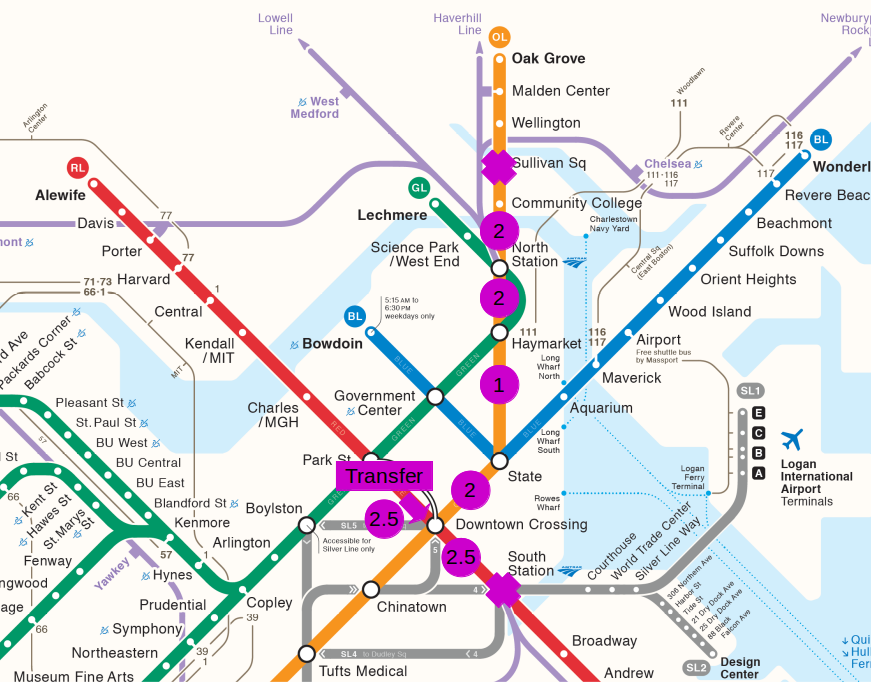
\includegraphics[scale=0.6]{transfer_with_markup}\end{center}

Each interstation time is added along with transfer time to get a total 'distance' from Sullivan Square to South Station of 12 minutes. After building a graph of all such transit and transfer times, I found all stations that could be reached within 15 or 30 minutes from the station of interest. I then summed the nearest data for all those stations, to prevent overlapping data between stations. The result will be referred to as the network data for each station. 

\subsection{Station Data Estimates}

Putting all these factors together, I create data estimates for each station and for each area calculation. For every station on the network, I estimate the population, number of housholds, employment, and total pay for the area that is nearst to each station, within walking distance of each station, with driving distance and nearest to each station, within a 15 minute transit trip from each station, and within a 30 mintue transit trip from each station. These 20 data points, along with the parking flag, comprise the feature set for this experiment. 






\end{document}